%\documentclass[preview, border=5mm]{standalone}
\documentclass[a3paper]{slides}

\usepackage[margin=1cm]{geometry}

% for the \xintFor***
\usepackage{xinttools} 
\usepackage{tikz}
\usetikzlibrary{calc}


% playing role of infinity (should be < .25\maxdimen)
\def\bigLen{20cm}

% define the "half plane" to be clipped (#1 = half the distance between cells)
\tikzset{
  half plane/.style={ to path={
       ($(\tikztostart)!.5!(\tikztotarget)!#1!(\tikztotarget)!\bigLen!90:(\tikztotarget)$)
    -- ($(\tikztostart)!.5!(\tikztotarget)!#1!(\tikztotarget)!\bigLen!-90:(\tikztotarget)$)
    -- ([turn]0,2*\bigLen) -- ([turn]0,2*\bigLen) -- cycle}},
  half plane/.default={2pt}
}

% number of random points
\def\puntosCantidad{30} 

% random points are in [-\maxX,\maxY]x[-\maxX,\maxY]
\def\maxX{ 13.85 }
\def\maxY{\maxX * 1.43}

\begin{document}

  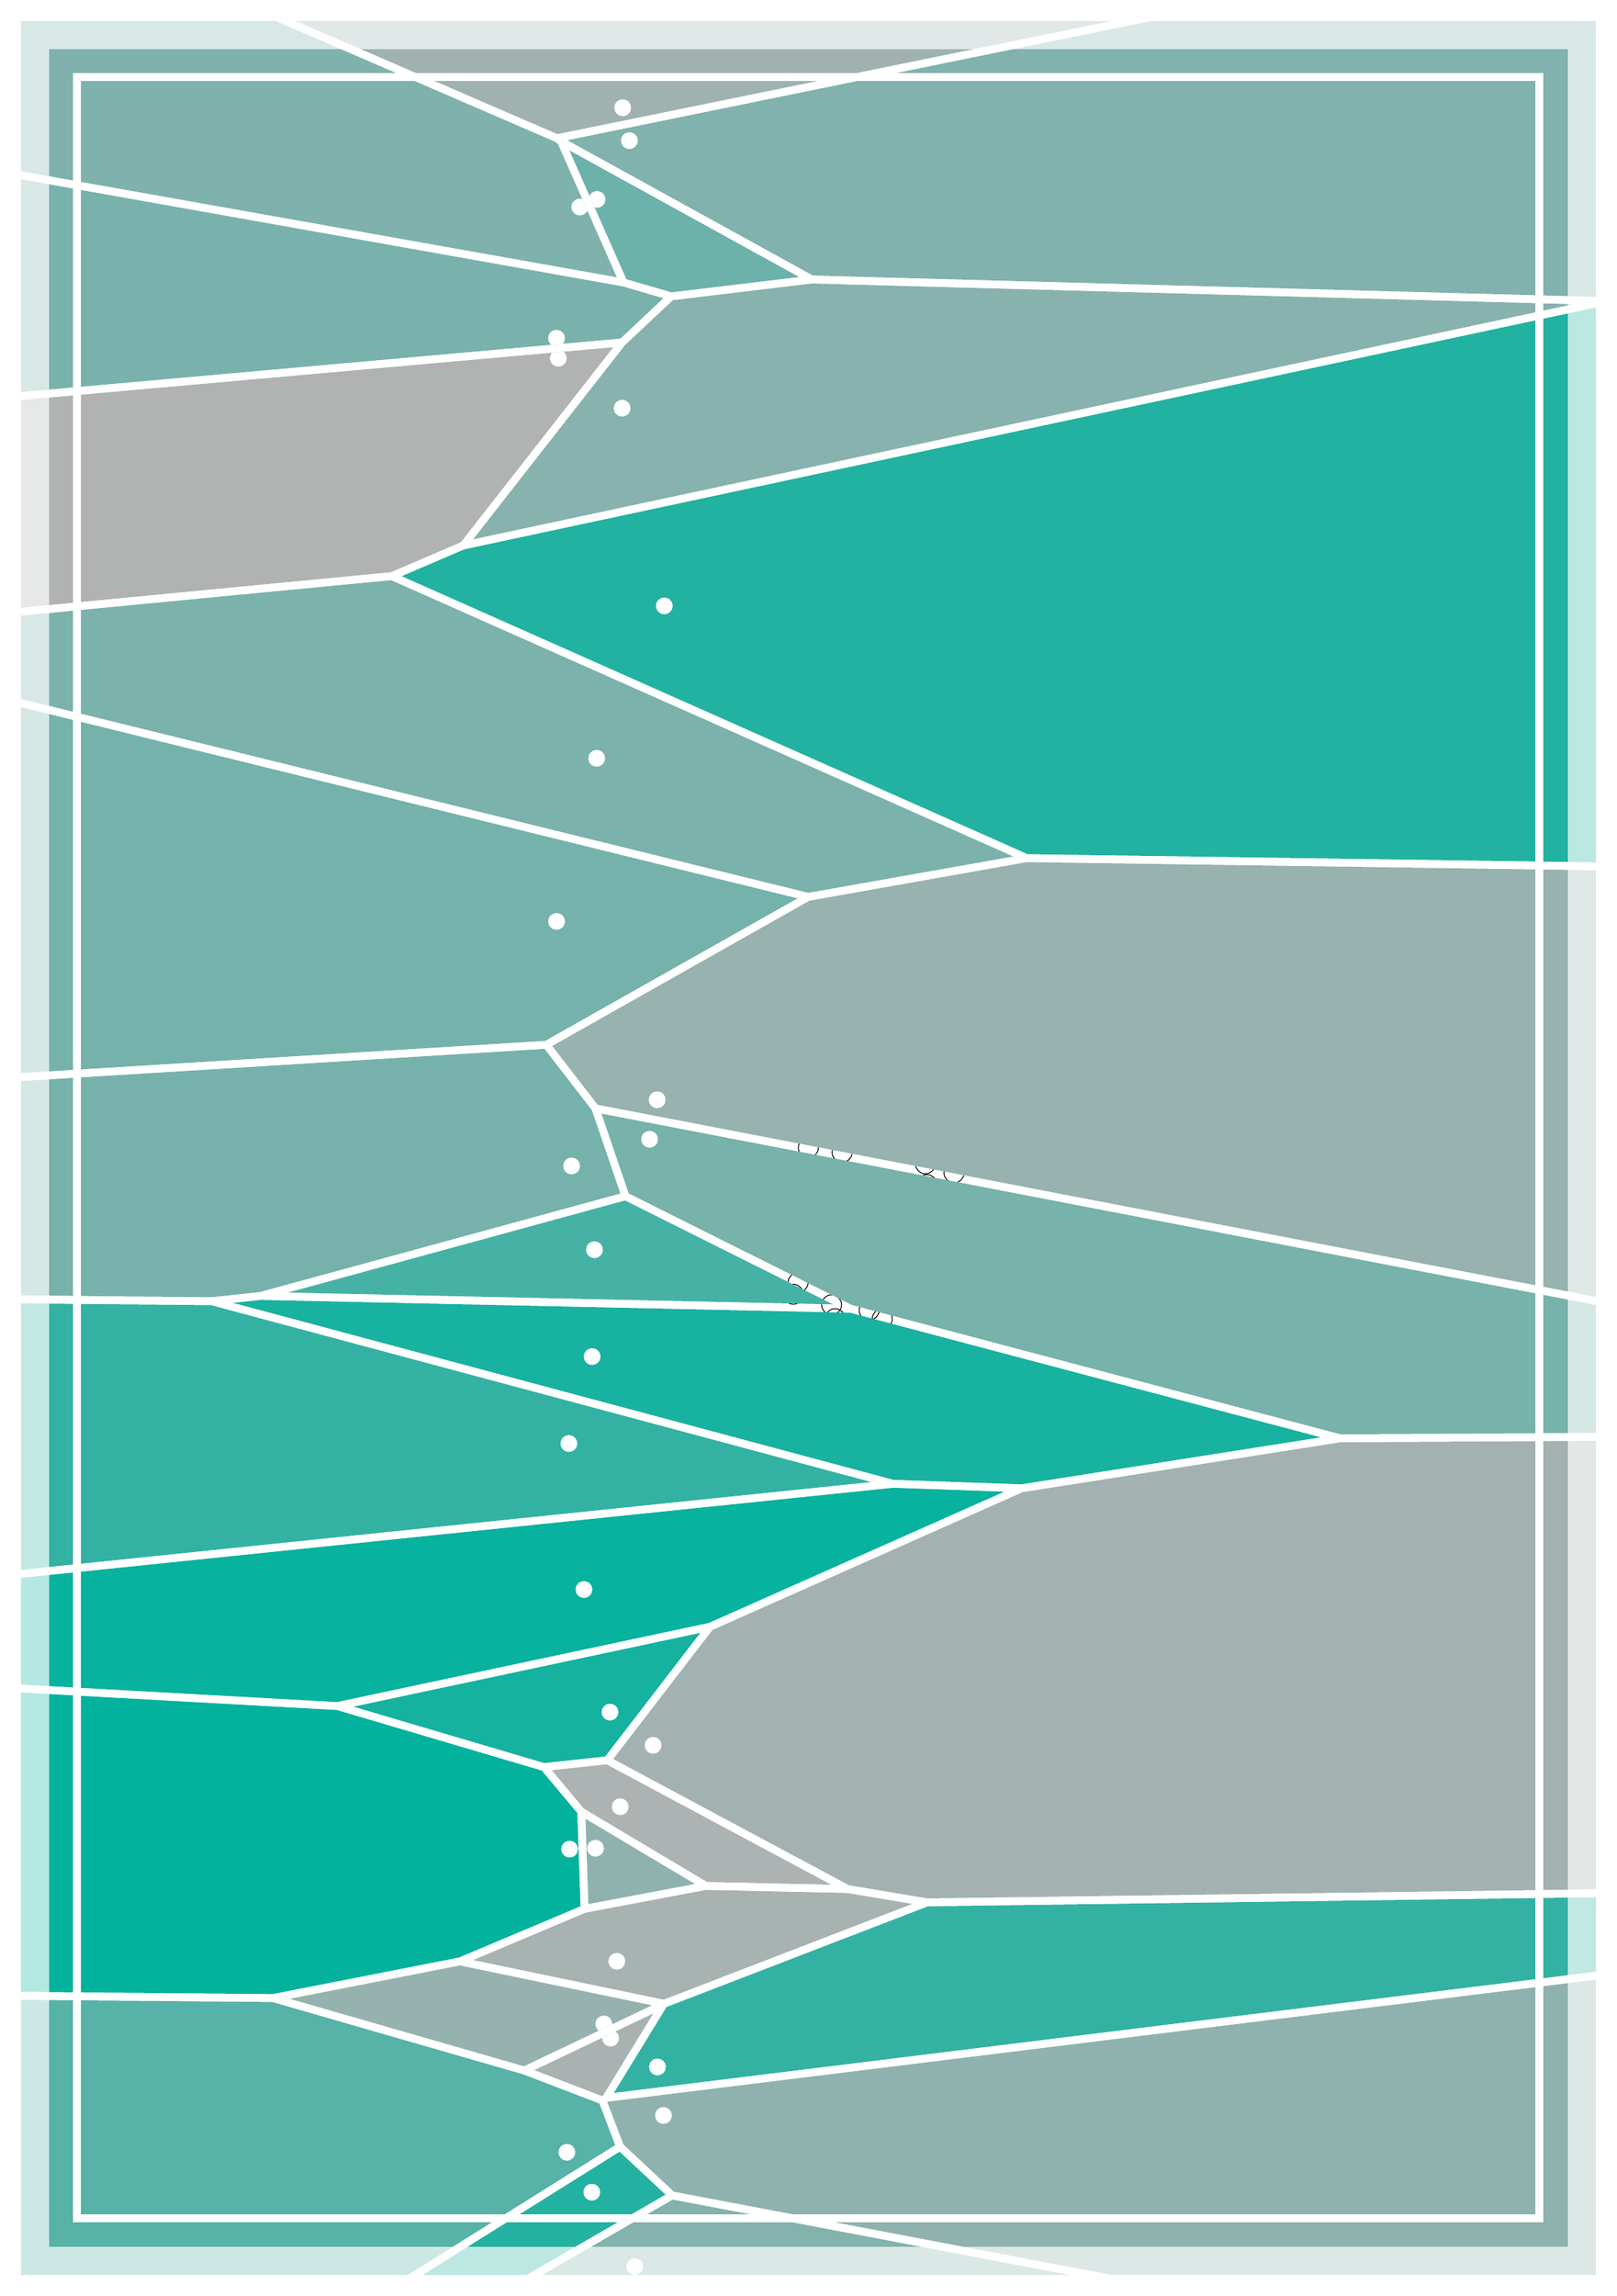
\begin{tikzpicture}

    % generate random points
    % \pgfmathsetseed{1908}
    \def\cuenta{1}
    \def\puntos{}
    \draw [fill=white] circle [radius=5pt] (0,0) \foreach \t in {1,2,...,\puntosCantidad}{
         ++( { sqrt( \t ) * 700 } : 2cm ) circle [radius=5pt]
    };
    \xintFor* #1 in { \xintSeq {1}{\puntosCantidad} } \do{

      % random x in [-.9\maxY,.9\maxY]
		  \pgfmathsetmacro{\puntoX}{ (-\maxX*0.25) + rand } 

      % random x in [-.9\maxY,.9\maxY]
	  \pgfmathsetmacro{\puntoY}{ \maxY * rand } 
	  \edef\cuenta{\cuenta + 1}
      % stock the random point
      \edef\puntos{\puntos, ( \puntoX, \puntoY )} 
    }

    % draw the points and their cells
    \xintForpair #1#2 in \puntos \do{
      \edef\puntoA{#1,#2}

      \begin{scope}
        \xintForpair \#3#4 in \puntos \do{
          \edef\puntoB{#3,#4}

          % check if (#1,#2) == (#3,#4) 
          \ifx\puntoA\puntoB\relax 
            \tikzstyle{myClip}=[];
          \else
            \tikzstyle{myClip}=[clip ];
          \fi;
          \path [myClip] (#3,#4) to [half plane] (#1,#2);
        }
        % last clip
        \clip (-\maxX,-\maxY) rectangle (\maxX,\maxY); 

        \pgfmathsetmacro{\randSat}{ rnd }
        \definecolor{randcolor}{hsb}{ .48, \randSat, .7 }
        % fill the cell with random color
        \fill[randcolor] (#1,#2) circle (14*\bigLen); 
        % and draw the point
        \fill[draw=white,fill=white] (#1,#2) circle (4pt); 
      \end{scope}

    }

    \draw[draw=white,line width=4pt] 
	  ({-\maxX + 1},{-\maxY + 1})
	  rectangle 
	  ({\maxX - 1},{\maxY - 1});
    \draw[draw=white,draw opacity=.7,line width=1cm] 
	  ({-\maxX },{-\maxY }) 
	  rectangle 
	  ({\maxX },{\maxY });


    %\draw  (0,0) \foreach \t in {0.1,0.2,...,10}{
    %  -- ++({sqrt(\t)*700}:2cm)
    %};
    %\draw [fill=white] circle [radius=5pt] (0,0) \foreach \t in {1,2,...,\puntosCantidad}{
    %     ++( { sqrt( \t ) * 700 } : 2cm ) circle [radius=5pt]
    %};

    \pgfresetboundingbox
	  \draw[draw=white] (-\maxX,-\maxY) rectangle (\maxX,\maxY );
  \end{tikzpicture}

\end{document}

% Source: https://tex.stackexchange.com/questions/138668/how-to-draw-and-paint-the-voronoi-regions-of-a-series-of-points-using-tikz

% Some comments on the code :
% 
% • Given two points, A and B, the points that are closer to A is a half plane,
%   delimited by the perpendicular bisector, and containing A.
% • So to construct the Voronoi cell of A we can take the intersection of all
%   this half planes when B runs over all other points (different from A).
% • In the code, taking this intersection is done by clipping big rectangles
%   that plays the role of "half planes".
% • I was not able to use \foreach because clipping inside such a loop is not
%   available outside the loop (\foreach creates a group). So I'm overcoming
%   this by using \xintFor.
% 
